\section{Empirical Results}
\label{sec:empirical-results}
To evaluate the algorithms presented in Section~\ref{sec:flexible-resource-allocation-mechanisms},
this section analyses the performance of both the greedy and auctions algorithms
(subsections~\ref{subsec:evaluation-of-the-greedy-algorithm} and~\ref{subsec:evaluation-of-the-auction-mechanisms}).
We investigate the effect of server heuristics on the Decentralised Iterative Auction
(subsection~\ref{subsec:effectiveness-of-decentralised-iterative-auction-heuristics}) and
the possibility of misreporting task attributes within the Decentralised Iterative Auction
(subsection~\ref{subsec:possibility-of-misreporting-task-attributes-in-decentarlised-iterative-auction}).
Finally we analyse the effectiveness of elastic resource allocation given server resource capacity ratios
(subsection~\ref{subsec:the-effective-of-elastic-resources-given-server-resource-capacity-ratio})
and the comparison between online and batched resource allocation methods
(subsection~\ref{subsec:comparison-between-online-and-batched-resource-allocation}).

Within Edge Cloud Computing, we have found no de facto standard for testing resource allocation algorithms and
those used in related work do not consider a deadline applicable for our work. Therefore we have generated synthetic
models for our servers and tasks. This is done using a handcraft Gaussian distribution for each attribute that can be
found in Appendix B\@.

In order to compare the results of the different algorithms, a branch and bound solution was implemented to solve
the optimisation problem, from subsection~\ref{subsec:optimisation-problem}. However due to the difficulty of
finding the optimal solution, this algorithm was only used in smaller settings were the optimal could be found within
a reasonable amount of time. \\
The settings chosen were 3 servers and 15 tasks, 6 servers and 30 tasks and 8 servers and 40 tasks where \~70\% of
tasks are allocated. \\
To compare to previous work that utilise a fixed resource requirement, each task's resource speeds were determined by
finding the minimum sum total of resource speeds according to the task deadline. This aims to give each task a
balanced amount of each resource making comparisons as fair as possible.

\subsection{Evaluation of the Greedy Algorithm}
\label{subsec:evaluation-of-the-greedy-algorithm}
In order to compare the greedy algorithm, the branch and bound solution above can be used to find the optimal solution
for both the flexible and fixed resource allocation methods. However as explained above, to use the time required we
are not able to use the solution for the larger problem setting (8 servers and 40 tasks). Therefore by modifying the
greedy algorithm to use a fixed resource allocation we are able to find an approximate solution for the fixed resource
allocation case in the large setting. \\
Along with this, a relaxed solution was implemented with the branch and bound algorithm containing just a single
server that combined all of the server capacities into one. The optimisation problem for it can be found in Appendix C\@.
This was used as the upper bound for the social welfare as the server is able to complete at least as much as all of the
servers individual as well as use the remaining resources of the servers to possible compute more tasks. \\
For the greedy algorithm, a wide range of possible functions were tested with the best found being - value density
function: \[\frac{v_j \cdot d_j}{s_j + w_j + r_j}\] server selection:
\[\text{argmin}_{\forall i \in I} S^{'}_i \cdot W^{'}_i \cdot R^{'}_i\] for task $j$ and servers $I$ and the resource allocation:
\[\text{argmin}_{s^{'}_j, w^{'}_j, r^{'}_j} \left(\frac{w^{'}_j}{W^{'}_i}\right)^3 + \left(\frac{s^{'}_j + r^{'}_j}{R^{'}_i}\right)^3\]
is task $j$ and server $i$.

\begin{figure}
    \centering
    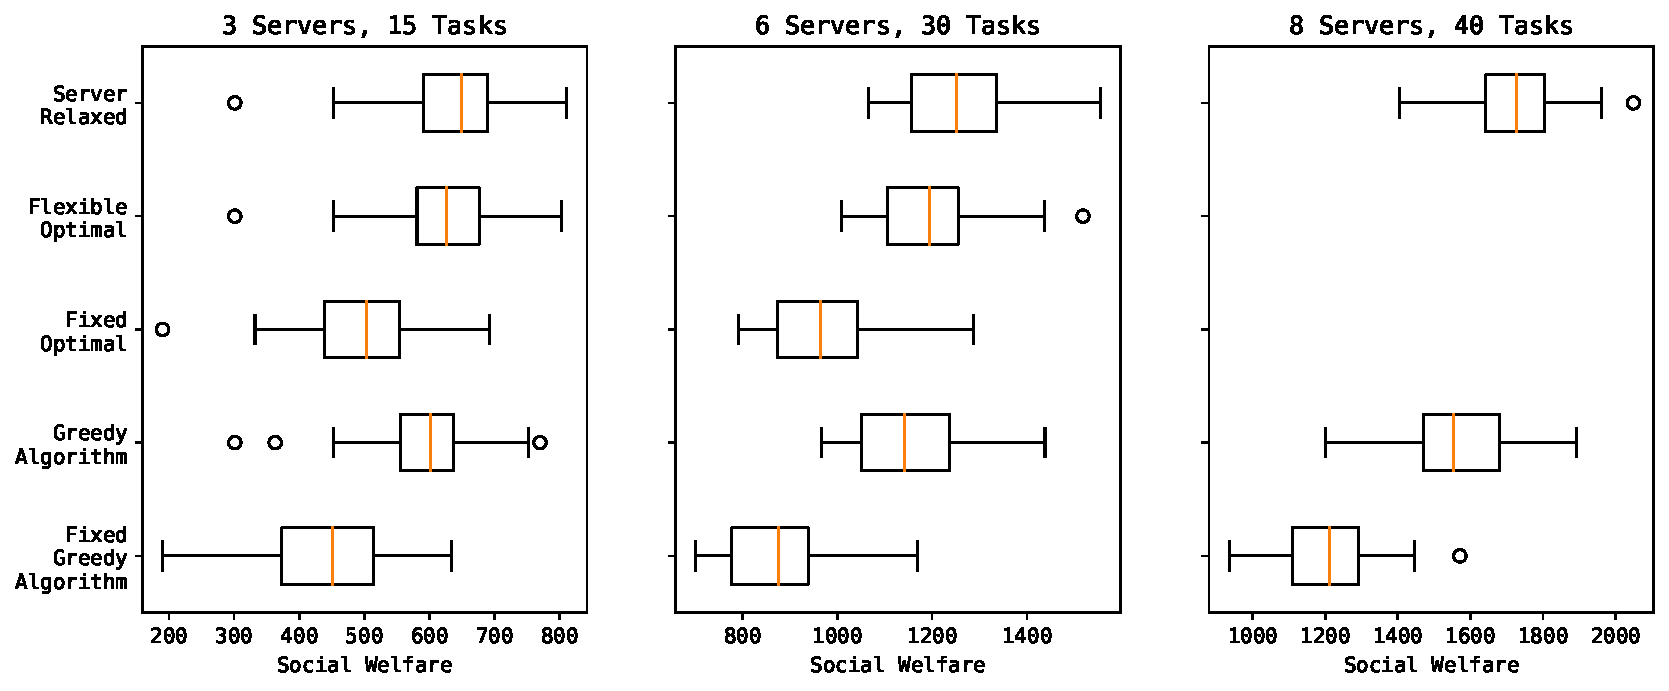
\includegraphics[width=\linewidth]{figs/greedy/multi_setting_social_welfare.pdf}
    \caption{Social welfare of the greedy algorithm, optimal flexible solution, optimal server relaxed solution,
             optimal fixed solution}
    \label{fig:greedy-algorithm-comparison}
\end{figure}
%% TODO Explain the results, percentage difference in social welfare with each algorithm and the difference
%% between the solutions for the optimal and approximation

\subsection{Evaluation of the Auction mechanisms}\label{subsec:evaluation-of-the-auction-mechanisms}
VCG, as explained in section~\ref{sec:flexible-resource-allocation-mechanisms}, is the traditional method of dealing
with self-interested users due to being incentive compatible. However, this requires solving the optimal solution
for each individual task making such a mechanism infeasible except for small setting. Because of this, VCG is used for
a comparison with the Critical Value Auction and Decentralised Iterative Auction in the smaller settings. \\
For the Critical Value Auction, the same function were used for the analyse of the greedy algorithm, in
subsection~\ref{subsec:evaluation-of-the-greedy-algorithm}. For the Decentralised Iterative Auction, the server
heuristics are a price change of 3 and an initial price of 25 for all servers. The reason for these heuristics over
others is explained in subsection~\ref{subsec:effectiveness-of-decentralised-iterative-auction-heuristics}.

\begin{figure}[h]
    \centering
    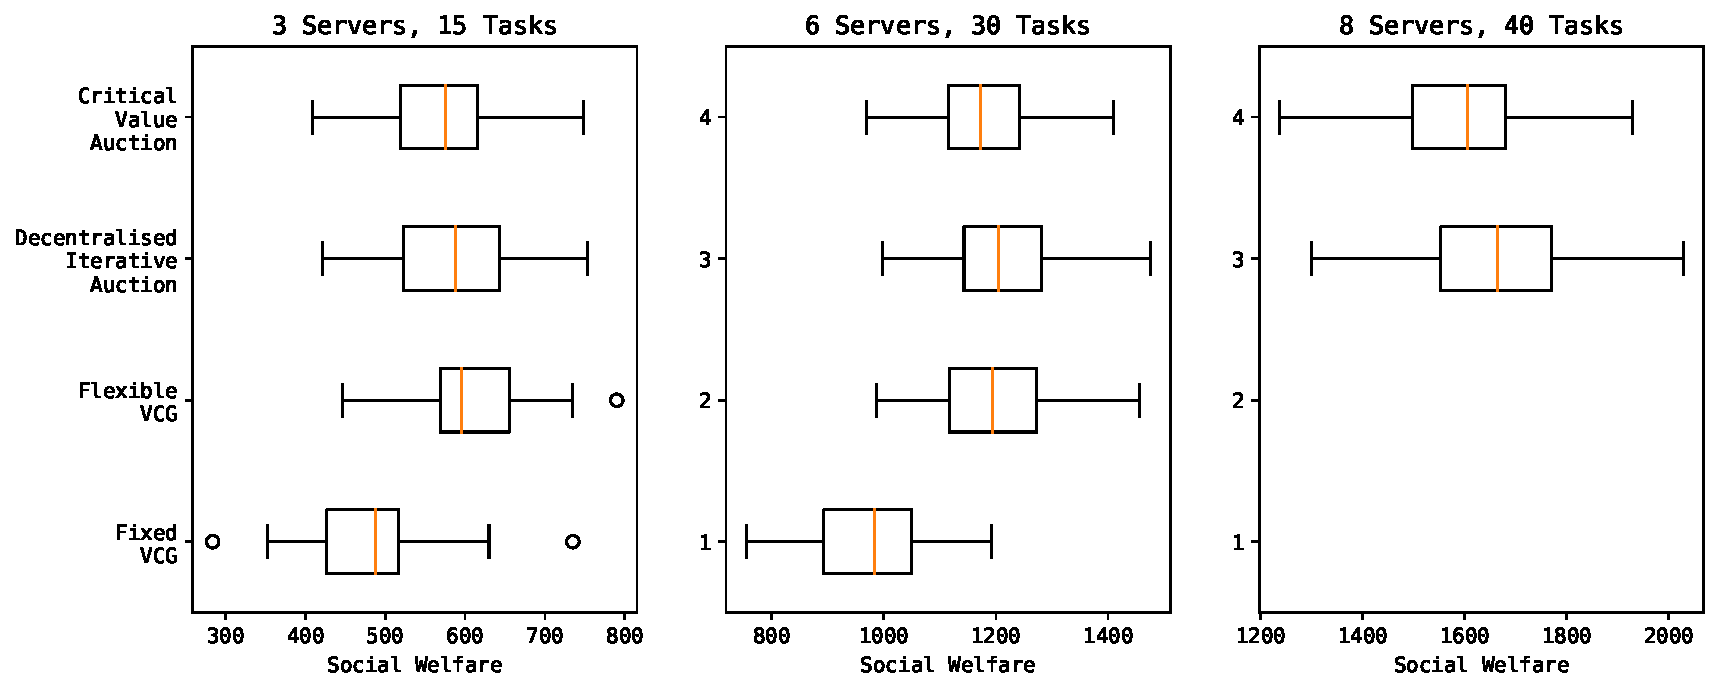
\includegraphics[width=\linewidth]{figs/auctions/multi_setting_social_welfare.pdf}
    \caption{Comparison of the social welfare for the auction mechanisms}
    \label{fig:auction-mechanisms-social-welfare}
\end{figure}

\begin{figure}[h]
    \centering
    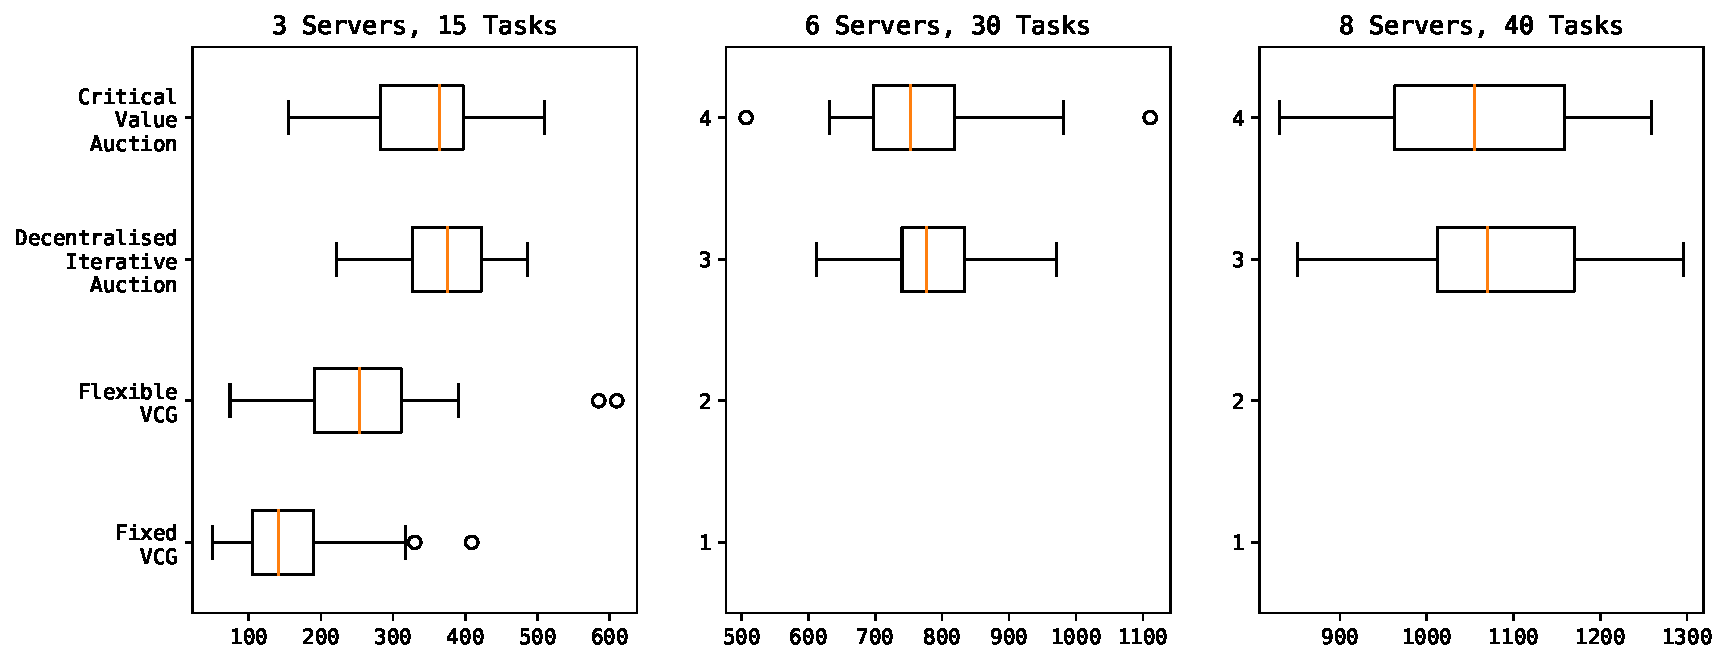
\includegraphics[width=\linewidth]{figs/auctions/multi_setting_revenue.pdf}
    \caption{Comparison of the social welfare for the auction mechanisms}
    \label{fig:auction-mechanisms-revenue}
\end{figure}

%% TODO explain the results, percentage difference in social welfare for the DIA and difference in revenue between
%%  algorithms

\subsection{Effectiveness of Decentralised Iterative Auction Heuristics}
\label{subsec:effectiveness-of-decentralised-iterative-auction-heuristics}
As explained in subsection~\ref{subsec:decentralised-iterative-auction}, the Decentralised Iterative Auction
calculates the price of task as the difference in revenue between the task being allocated (with a price of
zero) and not being allocated. To increase a server revenue, a server will increase the price by a value referred to as
the price change variable. \\
This is important as if a task has a value of 10 and the difference in revenue is 7 but the
price change is 4 then the resulting price is 11, above the task's value prevent it from being allocated. As a result,
the task won't be allocate to the server however if the price change was 3 then the task could have been allocated
resulting in the server's total revenue benefiting both the server and the task in question. \\
A second heuristic, the initial price variable, is used to speed up the auction and reduce the number of rounds by
aiming to set the price close to the task's actual value. This in turn reduces the number of rounds for the task price
to converge on the task value. However, a similar problem as the price change variable exists such that if the initial
price is greater than a tasks actual value then the task will never be allocated to a server. \\
Therefore the selection of price change and initial price can have a significant impact on the social welfare, revenue
and number of rounds the auction takes. As the mean value of tasks is 50 (see Appendix B),
the initial prices were set at 20, 25, 30, 35 and 40 while the price change variables were set at 1, 3, 5, 7, 10. These
values were chosen to allow for understanding the auction where value at both ends of the spectrum are used for both
variables, in order to see the effect on social welfare, revenue and number of rounds taken. For this case, we used
30 tasks and 6 servers.

\begin{figure}[h]
    \centering
    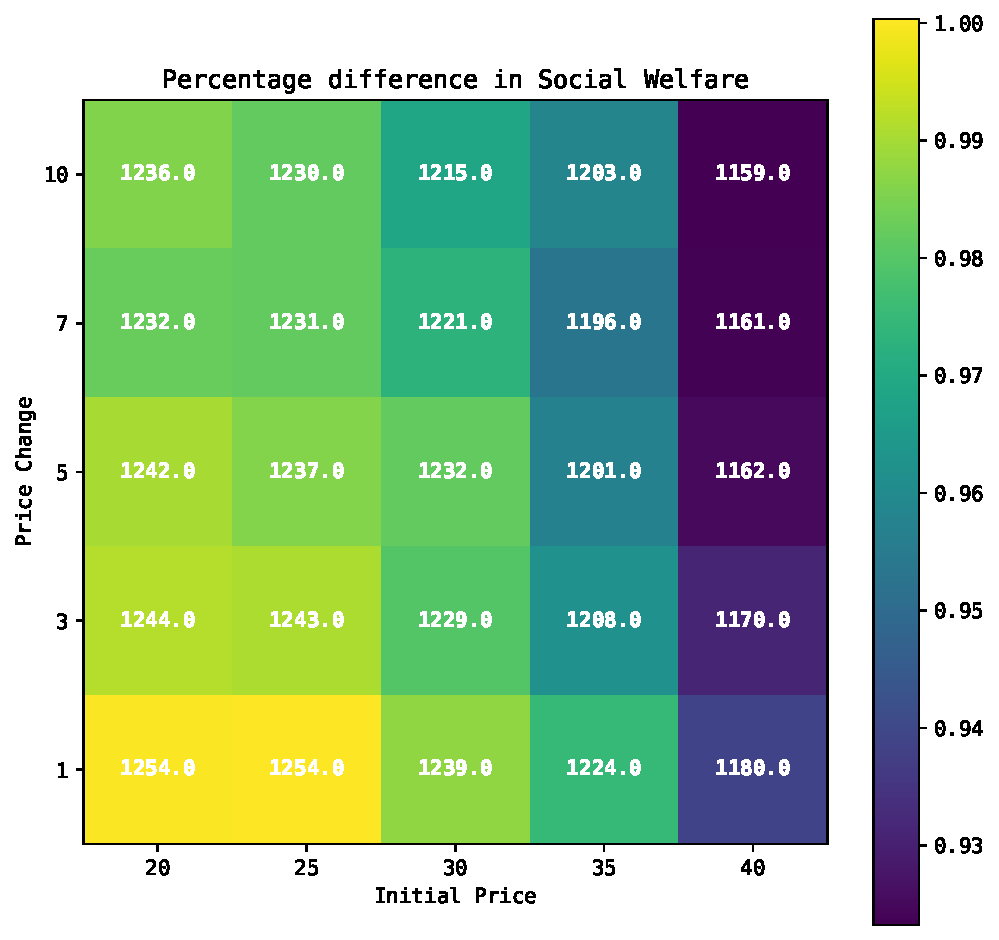
\includegraphics[width=0.45\linewidth]{figs/dia_heuristics/social_welfare_grid.pdf}
    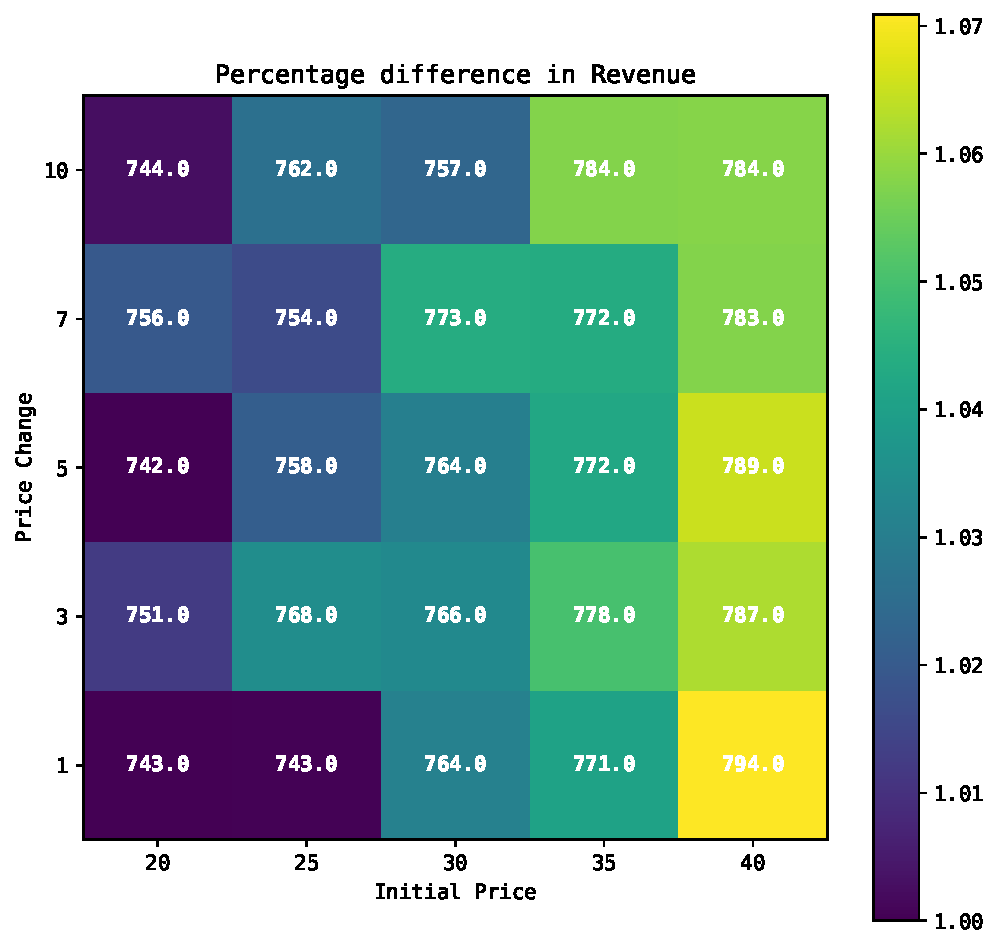
\includegraphics[width=0.45\linewidth]{figs/dia_heuristics/revenue_grid.pdf}
    \caption{Grid search of difference server price change and task initial cost effect on social welfare (left) and
             revenue (right)}
    \label{fig:dia-sw-rev-grid-search}
\end{figure}

%% TODO reread to make sure it makes sense
Figure~\ref{fig:dia-sw-rev-grid-search} maps a grid search of different price change and initial price values plotting
the social welfare on the left and the total revenue on the right. The value are normalised with the result of the
solution with a price change of 1 and initial price of 20. For the social welfare the percentage different between the
best case (price change of 1 and initial price of 20) to the worst results (price change of 10 and initial price of 40)
is only -7\% meaning that the auction is resilient to a range of price change and initial price values. \\
While interesting when measuring the revenue, the lowest revenue occurs for the case of price change of 1 and initial
price of 20. This is understandable as the system will arrive at a revenue local optima and for this case a majority of
tasks will pay their critical value however this also results in servers not gaining by forcing tasks by paying more
than they could have. However for the case with an initial price of 40, this forces tasks off the bat to pay a price of
40, in most cases more than their critical value.

Within the context of edge cloud computing, the number of rounds for the Decentralised Iterative Auction is important
to making it a feasible auction as the time taken is proportional to the number of rounds run.
Figure~\ref{fig:dia-rounds-grid-search} shows the number of rounds required on average for each heuristic. For the case where the
auction used the minimum heuristic values (price change of 1 and initial price of 20) that achieves the highest social
welfare comes at the close of requiring on average 400 rounds. This means that on average tasks require XX number %% TODO
of individual rounds to converge on a price. In comparison when the price change is set to 10 and the initial price is
kept at 20, the average number of rounds required is 5x less at 80.

This shows that the Decentralised Iterative Auction is an effective auction but has tradeoffs for server who must
choose whether to maximise social welfare, revenue or rounds as each requires a different selection of heuristics.

\begin{figure}[h]
    \centering
    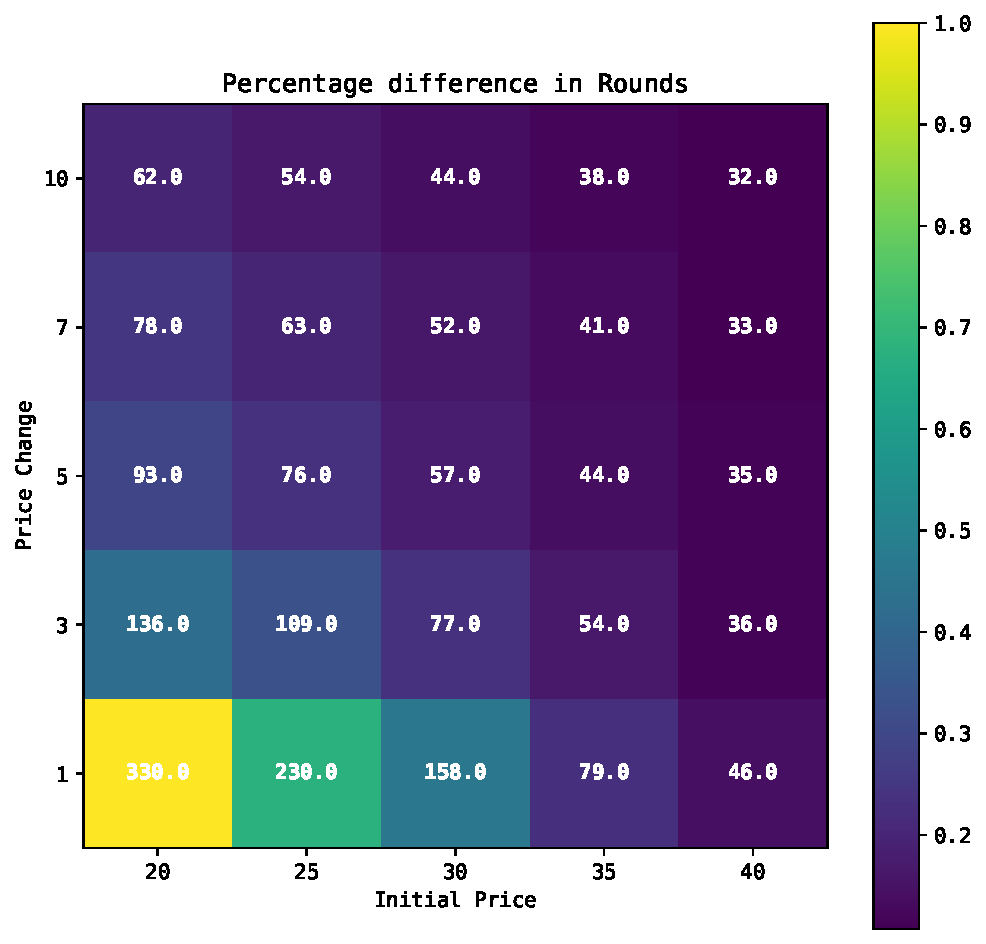
\includegraphics[width=0.45\linewidth]{figs/dia_heuristics/rounds_grid.pdf}
    \caption{Grid search of difference server price change and task initial cost effect on round count and number of
             task rounds}
    \label{fig:dia-rounds-grid-search}
\end{figure}

\subsection{The Possibility of Misreporting Task Attributes in Decentralised Iterative Auction}
\label{subsec:possibility-of-misreporting-task-attributes-in-decentarlised-iterative-auction}
In Subsection~\ref{subsec:decentralised-iterative-auction}, the Decentralised Iterative Auction was shown to be not
incentive compatible in specials cases however it is doubted that the ability for users to cheat more generally was
possible. Therefore, this problem was addressed by applying a grid search of task attributes and to randomly modify
individual tasks to investigate if tasks can pay less compared to if it didn't misreport.

For the random modification search, this was done by taking a random task and mutating each of the task's attributes.
% Todo Explain the grid search and random mutation results

\subsection{The Effective of Elastic Resources given Server Resource Capacity Ratio}
\label{subsec:the-effective-of-elastic-resources-given-server-resource-capacity-ratio}
The major advantage of using elastic resource allocation is to the control that it gives to servers. This becomes
increasing important if task requirements are unbalanced compared to server resource capacity. To measure the impact
of elastic resource allocation compared to fixed resource allocation, server computation and bandwidth capacities
are redistributed to different ratios in order to compare. The reason only the computation and bandwidth capacities
are modified is due to elasticity not affect the server's storage just its bandwidth and computation
(eq~\ref{eq:server-bandwidth-constraint} for loading and sending results and eq~\ref{eq:server-computation-constraint}
for computation results). \\
Server resources are redistributed using a percentage of the server's total (computation + bandwidth) resources.
This is shown as a ratio of server computation to bandwidth ratios in figures~\ref{fig:resource-ratio-social-welfare}
and~\ref{fig:resource-ratio-server-resource-usage}.

\begin{figure}[h]
    \centering
    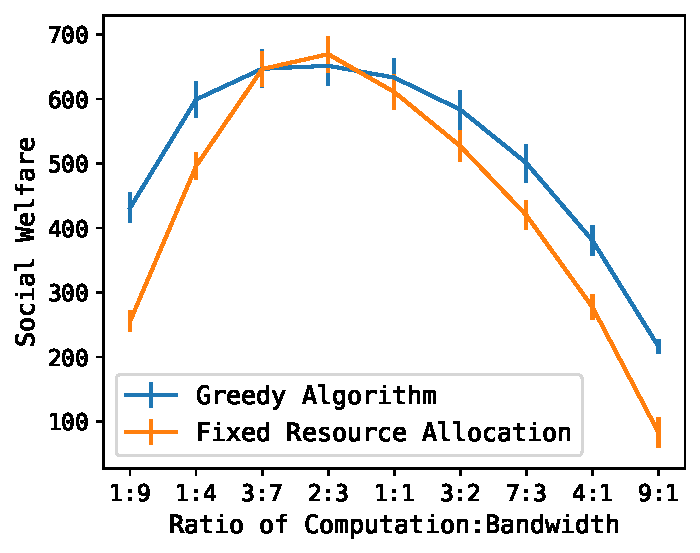
\includegraphics[width=0.45\linewidth]{figs/resource_ratio/social_welfare.pdf}
    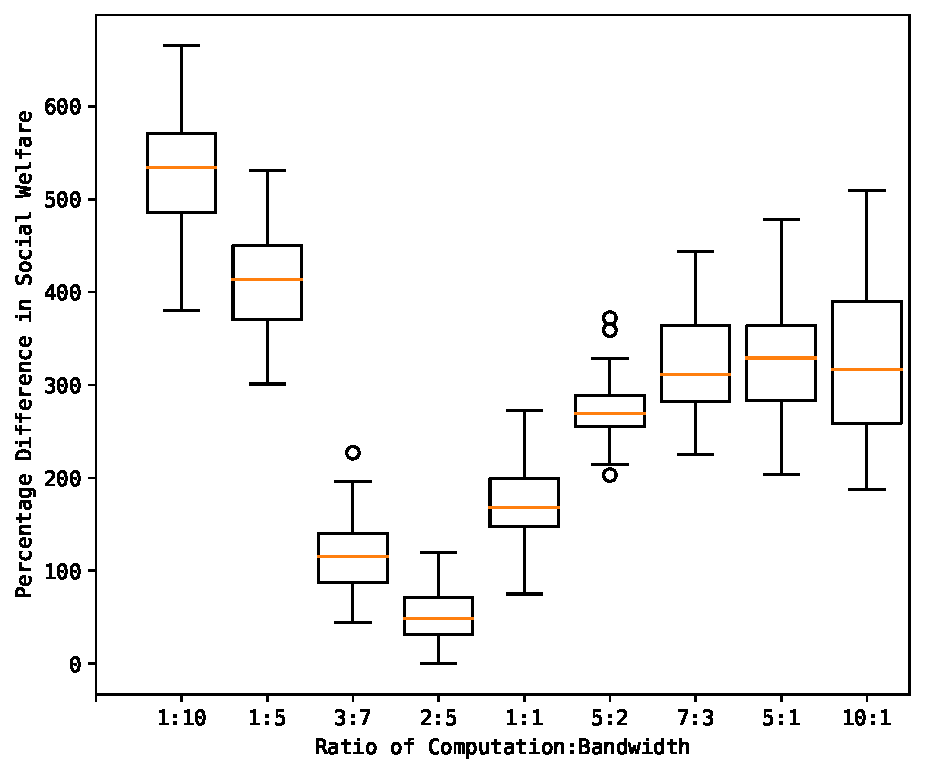
\includegraphics[width=0.45\linewidth]{figs/resource_ratio/social_welfare_difference.pdf}
    \caption{The effect of server resource ratios on average social welfare percentage and the social welfare difference}
    \label{fig:resource-ratio-social-welfare}
\end{figure}

Figure~\ref{fig:resource-ratio-social-welfare} is the combination of two graphs showing the same data. The left graph
shows the average social welfare achieved by the respective algorithms with different server resource ratios. As can be
seen on the figures at the ratio extremes, there is a significant difference in results between the flexible and fixed
resource allocation. This can be seen more clear by the right graph, that plots the difference in social welfare per
model with the error bars. \\
This observation is important for Edge Computing as nodes may have a large discrepancy in server resource capacity
due several reasons, i.e. a persistence task running over a long period of time, internet connection issues limiting
overall bandwidth, etc. For these cases, the elasticity of tasks has a significant boost to the number of tasks and
in social welfare in comparison to fixed resource allocation.

\begin{figure}[h]
    \centering
    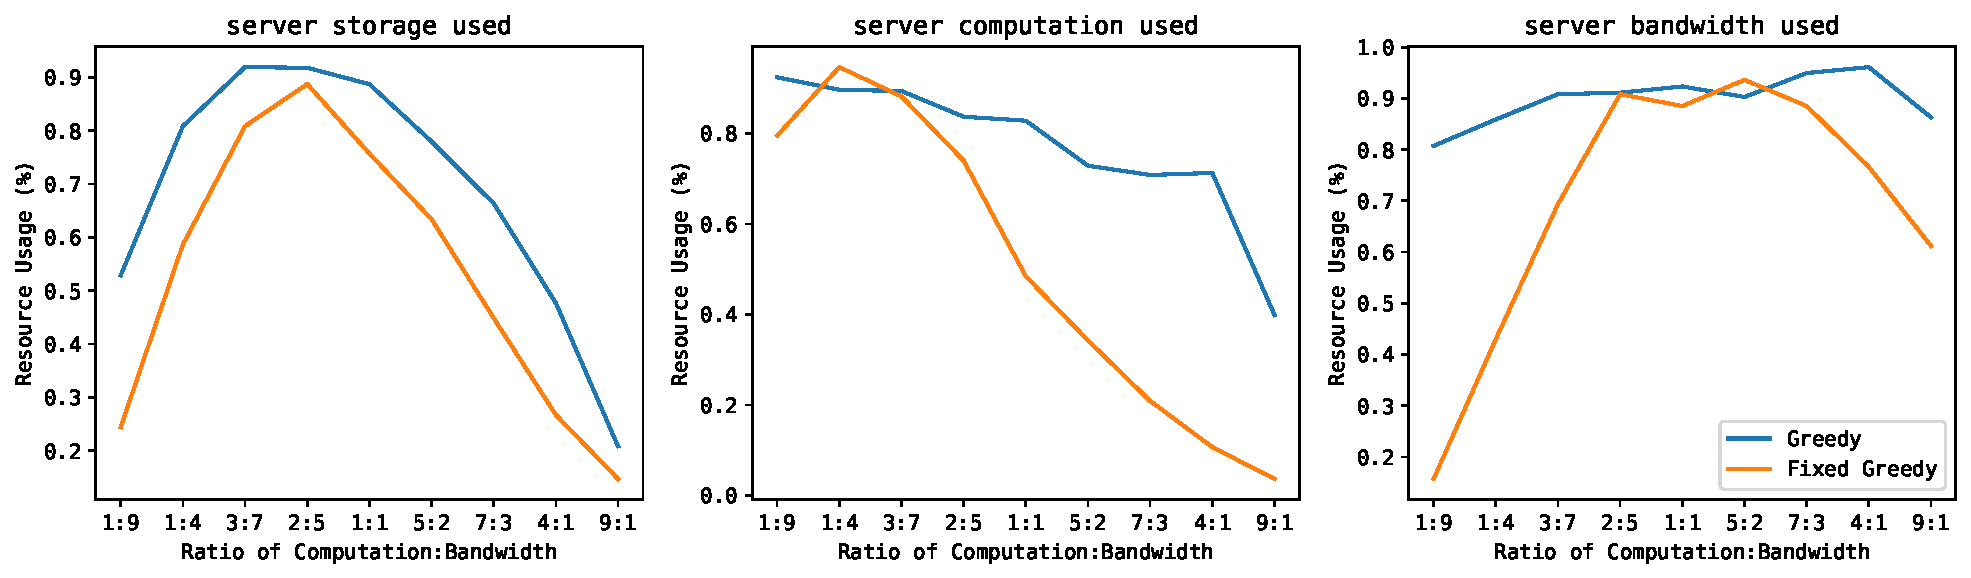
\includegraphics[width=\linewidth]{figs/resource_ratio/server_resource_usage.pdf}
    \caption{Server resource usage}
    \label{fig:resource-ratio-server-resource-usage}
\end{figure}

The effect of the redistribution of resources can be seen through the usage of resources by the servers per
each ratio in figure~\ref{fig:resource-ratio-server-resource-usage}. For cases where there is a large capacity of a
resource available, for elastic resource allocation these resources are able to be used to maximise the number of tasks
that can be run. This is particularly true of bandwidth as for a majority of the ratios, it is limiting factor for
allocating tasks.

\subsection{Comparison between Online and Batched Resource Allocation}
\label{subsec:comparison-between-online-and-batched-resource-allocation}
The purpose of this work has to be explore to use of elastic resource allocation in a static one-shot environment
meaning that all tasks arrive at the start, that are then allocated. However a problem exists with this formulation
that in reality, task do arrive over time. Section~\ref{sec:problem-formulation} proposed tasks are run in batches
overtime allowing no modifications to the algorithms proposed. This means that that as tasks arrive they are added to a
queue, such that when a new batch occurs, all of the tasks in the queue can be processed using the proposed algorithms
with no modifications. \\
Therefore choosing the right branch length is important as the more competition means better selection of tasks
increasing social welfare while the longer the branch length reduces the length of the task processing time. For the
Decentralised Iterative Auction, it has an advantage practically of being run in a batch as the auction doesn't need to
wait for all of the tasks to arrive compared to the Critical Value Auction. Therefore the auction can run during the
batch time frame with the task allocation at the end of the batch being the allocation.

We choose the batch lengths: 1, 2, 3, 4 because the mean length of a task is 10, any longer than this would result in
tasks on average tasks having to be computed in half their possible time. Plus, as can be seen in
figure~\ref{fig:batch-task-allocation}, the total social welfare decreases as the batch lengths increase investigating
longer batch lengths unwarranted.

\begin{figure}[h]
    \centering
    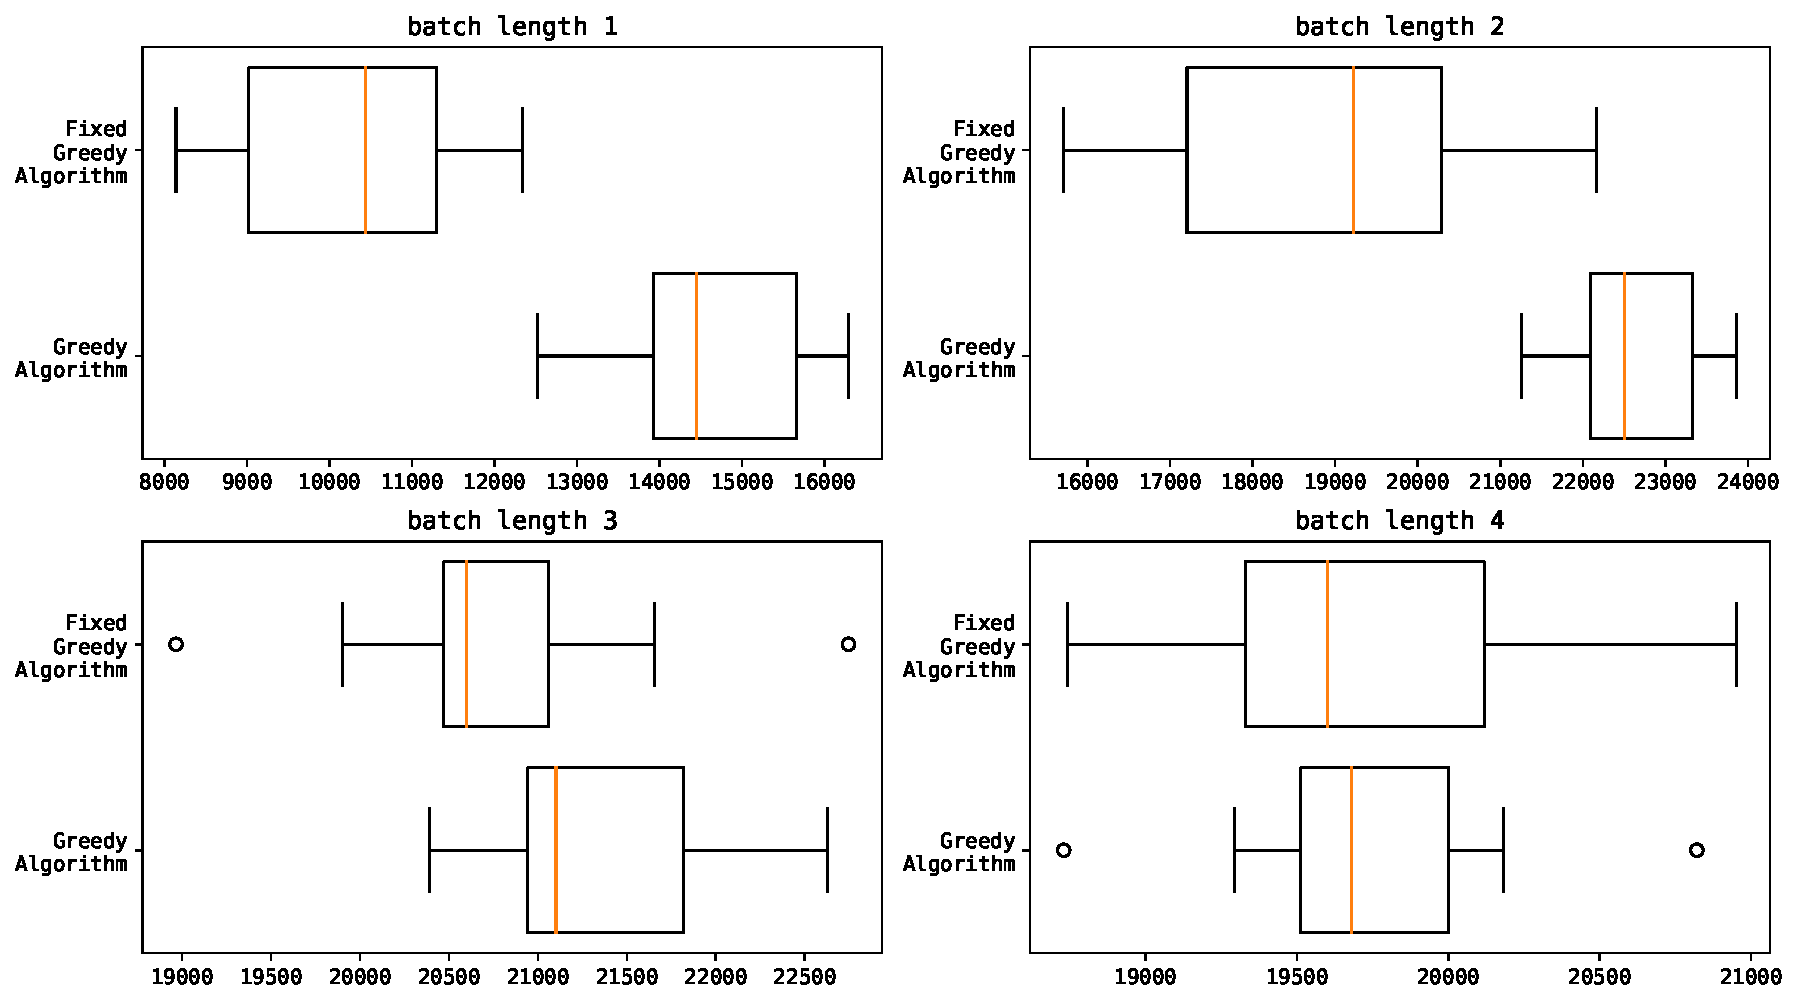
\includegraphics[width=\linewidth]{figs/online/online_batch_lengths.pdf}
    \caption{Online batch lengths}
    \label{fig:batch-task-allocation}
\end{figure}

%% TODO explain results